\documentclass{article}
\usepackage{iclr2024_conference,times}
\usepackage{booktabs,graphicx,amsmath,hyperref,url}
\usepackage{listings,xcolor,tikz,pgfplots}
\usetikzlibrary{arrows.meta,positioning}
\pgfplotsset{compat=1.18}
\hypersetup{colorlinks=true,linkcolor=blue,citecolor=blue,urlcolor=blue}
\lstset{basicstyle=\ttfamily\scriptsize,breaklines=true,columns=fullflexible,frame=single,showstringspaces=false}
\iclrfinalcopy
\title{Prompting a Data Quality Judge:\\Three Techniques and an Inspection Agent}
\author{CSC5051 Natural Language Processing\\Assignment 2 -- Task 3}
\begin{document}
\maketitle
\lhead{CSC5051 Assignment 2: Prompt Engineering \& Agents}
\begin{abstract}
This project treats instruction-tuning data selection as a four-criterion judgment with a conservative keep/review/reject policy. It compares zero-shot, two-example few-shot, and zero-shot stepwise prompting with a bounded inspection agent and a no-feedback ablation. All five conditions use the same 64 held-out records: 32 unaltered GPT-4 Alpaca examples and 32 explicitly constructed defects. The experiment measures defect rejection, original retention, paired discrimination, schema reliability, latency, and token cost. Unaltered records have no human quality labels; consequently, retention is not accuracy and a selected subset is not independently certified clean data. The study tests prompt and workflow behavior, not downstream training gains.
\end{abstract}

\section{Task, data, and quality policy}
\paragraph{Problem.} Task 3 asks for a quality evaluator that turns instruction-tuning data $D$ into a selected subset $D'$. An LLM can interpret semantic constraints that simple format filters miss, but its judgments can be inconsistent or unsupported. For each triple $x=(\text{instruction},\text{input},\text{output})$, the evaluator returns four scores and a brief reason. The deliverable implements $D'_m=\{x\in D: d_m(x)=\mathrm{keep}\}$ for each method $m$. Records assigned review are withheld for later adjudication. No training or parameter updates are performed.

\paragraph{Source and split.} The original English GPT-4 Alpaca file contains 52,002 triples \citep{peng2023}. We pin commit \texttt{38b93b75a80b019cc3aad362ca6f5bb0c3908959} and verify its SHA-256 before sampling. To bound API use, eligible records have instruction length 20--400 characters, input at most 600, output 60--800, combined length at most 1,400, and at least 95\% ASCII characters. Instructions containing repeat/repetition/echo/copy/nothing/blank/empty/silence are excluded. After deduplicating instruction--input pairs, 25,117 eligible records remain. Seed 20261028 selects 40 bases: eight for development and 32 for test. Length and language filters limit representativeness. The data are used for noncommercial coursework under CC BY-NC 4.0.

\paragraph{Controlled diagnostics.} Each base is paired with one synthetic defect: an empty output; an unrelated donor response with no overlap in filtered content words; the instruction/input echoed as the response; or the original response repeated four times. Each defect has eight test examples. Donors exclude the selected 40 bases. The resulting test has 64 rows, with labels and source identifiers hidden from prompts and tools. A four-pair development subset (eight rows) is used for the pilot. Unaltered examples are \emph{not} labeled good. Defect labels are operational constructions, not human annotations of naturally occurring errors; lexical separation does not itself prove semantic unrelatedness.

\paragraph{Rubric and decision.} The four dimensions are instruction following, correctness, relevance/completeness, and clarity. These capture compliance, trustworthiness, usefulness, and readability; they are project choices rather than a teacher-prescribed rubric. Scores are 0 (fails), 1 (partially meets), 2 (meets), or null (cannot assess). The shared deterministic policy is
\[
d(x)=\begin{cases}
\mathrm{reject},& \exists j:s_j=0,\\
\mathrm{keep},& \forall j:s_j=2,\\
\mathrm{review},& \text{otherwise, including unresolved nulls.}
\end{cases}
\]
Thus a minor defect scored 1 is reviewed rather than rejected, and unverifiable claims need not be guessed. Empty optional input is not itself an error. Strict parsing requires exactly the score keys, a lowercase decision consistent with the scores, and a nonempty reason. Invalid responses remain failures; they are never converted into favorable decisions.

\section{Prompts and the inspection agent}
All conditions share the rubric, strict JSON contract, and a system instruction to treat record contents as untrusted data. Only the three text fields reach the model. Exact templates are in the code supplement; Appendix~\ref{sec:examples} gives concrete examples and the common contract.

\paragraph{Zero-shot.} A direct request asks the model to evaluate the triple against the rubric without demonstrations. This is a short, low-complexity baseline.
\paragraph{Few-shot.} Two hand-authored addition examples illustrate a keep case ($2+3=5$) and a reject case ($2+3=7$), with scores and reasons. They are independent of all sampled records. In-context demonstrations aim to calibrate format and score meaning \citep{brown2020}; their narrow arithmetic domain is a limitation, and no demonstration covers review or null.
\paragraph{Stepwise / zero-shot CoT.} The prompt asks the model to identify task constraints, assess each criterion, check contradictions and unsupported claims, then apply the decision rule. This is a zero-shot stepwise adaptation \citep{kojima2022}, not a reproduction of rationale-demonstration CoT \citep{wei2022}. Only a concise justification is collected. Provider thinking is disabled in every condition; a stepwise instruction does not establish what internal reasoning the model actually performed.

\paragraph{Bounded agent.} The ReAct-inspired workflow \citep{yao2023} selects \texttt{finish}, \texttt{inspect}, or \texttt{reassess}, with at most three model calls. The final development prompt requires inspection for empty output, output exceeding 120 words (or uncertain near-threshold length), or apparent sentence/paragraph repetition. Other records may finish immediately or reassess. The model selects the action from the record; Python executes it and returns feedback. Inspection reports empty fields, character counts, word count, unique-word ratio, and the maximum word repetition count. It cannot verify facts or supply labels. After inspection, the model consumes the observation and finishes or reassesses; it is instructed not to inspect twice. Reassessment supplies no new evidence. Failure to finish within the call limit is invalid. This combines conditional tool use with a bounded loop, rather than giving every record an identical sequence of calls.

\begin{figure}[ht]
\centering
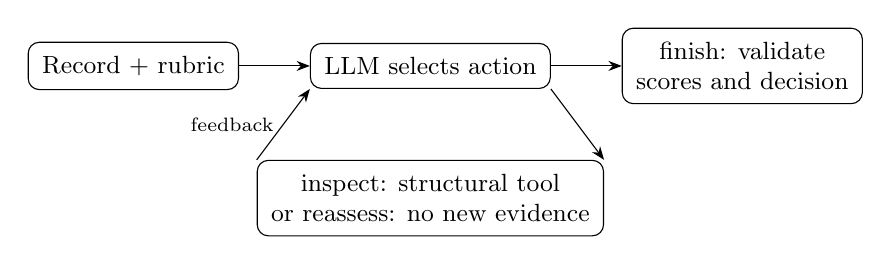
\begin{tikzpicture}[node distance=9mm, every node/.style={font=\small}, box/.style={draw,rounded corners,align=center,inner sep=5pt}, >=Stealth]
\node[box] (record) {Record + rubric};
\node[box,right=of record] (judge) {LLM selects action};
\node[box,right=of judge] (finish) {finish: validate\\scores and decision};
\node[box,below=of judge] (tool) {inspect: structural tool\\or reassess: no new evidence};
\draw[->] (record)--(judge);
\draw[->] (judge)--(finish);
\draw[->] (judge.south east)--(tool.north east);
\draw[->] (tool.north west)--node[left,font=\scriptsize]{feedback}(judge.south west);
\end{tikzpicture}
\caption{The bounded agent loop. A separate no-feedback condition replaces inspection observations with a withholding message; all other prompt and call-limit settings match.}
\end{figure}

\paragraph{Development decisions.} The first pilot produced 37 valid judgments out of 40: three CoT decisions used uppercase \texttt{Reject}. All 16 agent/ablation judgments finished without tools. We clarified the lowercase enum in the common contract and introduced the conditional inspection policy above. The second pilot produced 40/40 valid judgments, including two inspection branches in each agent condition. Both pilot versions and failures are retained. No held-out results were used to refine prompts; the final prompts and configuration were frozen before the test run.

\section{Experiment and results}
\paragraph{Controlled settings.} Actual inference used Volcengine Ark, returning \texttt{deepseek-v4-1-flash-260910}, on 28 October 2026. All conditions used temperature 0, \texttt{reasoning\_effort=none}, a 768-token completion cap, and the same record order. Three worker threads processed the five-method matrix; baselines use one call, agents up to three. Temperature 0 does not guarantee remote determinism. There is one held-out run per condition; timing includes network/provider variation and is not a controlled systems benchmark.

\paragraph{Metrics and denominators.} Original retention is keep/32; diagnostic rejection is reject/32; paired discrimination counts the 32 bases for which the original is kept \emph{and} its defect rejected. Review counts and all invalid/error outcomes remain visible. A reviewed defect is excluded from $D'$ but is not a successful rejection. These measures deliberately avoid treating originals as gold positives. Latency sums request times per record; it is not total experiment wall time. Costs use a conservative peak list rate of CNY 2/M input and 8/M output tokens, ignoring off-peak/cache discounts \citep{arkprice}.

\begin{table}[ht]
\centering\small
\begin{tabular}{lrrrrrrr}
\toprule
& Valid & \multicolumn{3}{c}{Originals (32)} & \multicolumn{2}{c}{Diagnostics (32)} & Paired\\
Method & /64 & Keep & Review & Reject & Reject & Review & /32\\
\midrule
Zero-shot & 64 & 25 & 5 & 2 & 27 & 5 & 20 \\
Few-shot & 64 & 27 & 4 & 1 & 25 & 7 & 21 \\
Stepwise CoT & 64 & 25 & 5 & 2 & 25 & 7 & 20 \\
Agent & 63 & 27 & 4 & 1 & 27 & 4 & 23 \\
No feedback & 63 & 27 & 4 & 1 & 27 & 4 & 22 \\
\bottomrule
\end{tabular}
\caption{Held-out results, using fixed denominators. No method kept a diagnostic. Each agent condition has one invalid diagnostic (excluded from reject/review counts but retained in denominators). Paired means keep original and reject its paired defect; originals are not gold positives.}\label{tab:quality}
\end{table}

\paragraph{Quality tradeoffs.} Zero-shot rejected 27/32 diagnostics (84.4\%) and kept 25/32 originals (78.1\%). Few-shot kept two more originals but rejected two fewer diagnostics. Stepwise prompting matched zero-shot original decisions exactly and moved two repetitive diagnostics from reject to review. The agent kept 27/32 originals and rejected 27/32 diagnostics, with the highest paired count (23/32, 71.9\%). That count does not establish better natural-data accuracy: it rewards original retention without gold quality labels. All five strict-policy subsets excluded every diagnostic; the unresolved distinction was often rejection versus review.

\paragraph{Which defects were difficult?} Every method rejected all eight empty, eight unrelated, and eight instruction-echo outputs. Differences occurred on excessive repetition (Figure~\ref{fig:repeat}). Review rather than reject can reflect a clarity score of 1, even when the explanation notices the repetition. This is a threshold/severity issue, not necessarily failure to notice the defect.

\begin{figure}[ht]
\centering
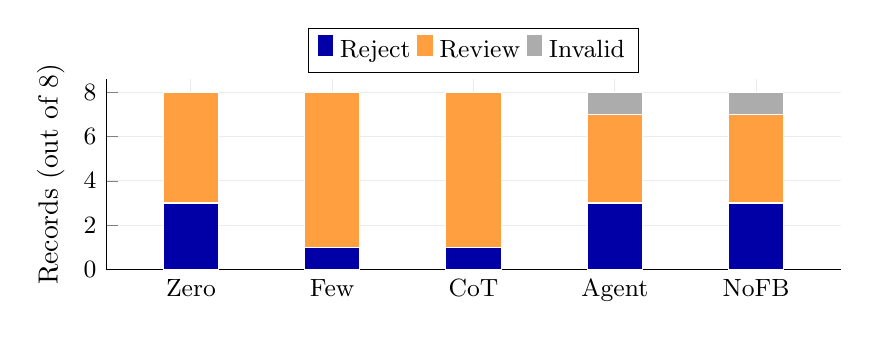
\begin{tikzpicture}
\begin{axis}[ybar stacked,width=.9\linewidth,height=4.0cm,
 ymin=0,ymax=8.6,ytick={0,2,4,6,8},ylabel={Records (out of 8)},
 symbolic x coords={Zero,Few,CoT,Agent,NoFB},xtick=data,
 bar width=20pt,enlarge x limits=.15,
 legend style={at={(.5,1.03)},anchor=south,legend columns=3,font=\small},
 axis lines*=left,tick label style={font=\small},grid=major,grid style={gray!15}]

\addplot[fill=blue!65!black,draw=white] coordinates {(Zero,3) (Few,1) (CoT,1) (Agent,3) (NoFB,3)};
\addplot[fill=orange!75,draw=white] coordinates {(Zero,5) (Few,7) (CoT,7) (Agent,4) (NoFB,4)};
\addplot[fill=gray!65,draw=white] coordinates {(Zero,0) (Few,0) (CoT,0) (Agent,1) (NoFB,1)};
\legend{Reject,Review,Invalid}
\end{axis}
\end{tikzpicture}
\caption{Outcomes on eight fourfold-repetition diagnostics. No repetition record was kept. NoFB denotes the agent without inspection observations.}\label{fig:repeat}
\end{figure}

\paragraph{Agent and ablation.} The agent inspected 18/64 records; the ablation inspected 17/64. No reassess action was observed and neither used a third call. The instruction to inspect was a prompt policy, not a runtime-enforced rule: both variants skipped three records whose actual whitespace word counts exceeded 120 (123, 124, and 131 words). The agent and ablation had identical aggregate keep/review/reject/failure counts, but differed on three diagnostic decisions and one paired success. One agent finish and one ablation finish omitted a closing JSON brace. Their plausible-looking assessments remain invalid, rather than being repaired after observing test results. The evidence supports an active feedback loop, but not a reliable overall benefit from feedback.

\begin{table}[ht]
\centering\small
\begin{tabular}{lrrrrrr}
\toprule
Method & Calls & Input tokens & Output tokens & Mean s & Median s & CNY\\
\midrule
Zero-shot & 64 & 34,519 & 5,259 & 1.40 & 1.34 & 0.1111 \\
Few-shot & 64 & 47,191 & 4,470 & 1.28 & 1.25 & 0.1301 \\
Stepwise CoT & 64 & 37,655 & 5,419 & 1.39 & 1.34 & 0.1187 \\
Agent & 82 & 78,286 & 6,655 & 1.80 & 1.56 & 0.2098 \\
No feedback & 81 & 76,100 & 6,560 & 1.77 & 1.50 & 0.2047 \\
\bottomrule
\end{tabular}
\caption{All 64 terminal records per method, including invalid outputs. Request latency is summed within a record. Costs use conservative list rates and include failed-format calls.}\label{tab:cost}
\end{table}

\paragraph{Cost and complexity.} The held-out run made 355 calls and cost an estimated CNY 0.774406. Including both pilots and the initial hello call, cumulative estimated spend was CNY 0.948306 against a CNY 10 ceiling; no uncertain reservations remain. These are list-rate estimates, not invoices. Relative to zero-shot, the agent cost 88.8\% more and mean record latency was 28.6\% greater. Its tool execution, bounded action parsing, trace storage, and multi-call state also add implementation complexity. On this study alone, zero-shot is a reasonable low-cost starting point; the higher paired agent count warrants broader validation before adoption.

\paragraph{Post-hoc threshold sensitivity.} Keeping all non-null scores at least 1 and total score at least 7 admits more originals but also repetitive diagnostics (Table~\ref{tab:threshold}). The weakest policy keeps any record with four non-null scores at least 1. These are deterministic reclassifications of existing scores, not new API runs or tuned test prompts. Invalid outputs remain excluded.
\begin{table}[ht]
\centering\small
\begin{tabular}{lrrr}
\toprule
Method & Strict all 2 & Sum $\geq7$, all $\geq1$ & All $\geq1$\\
\midrule
Zero-shot & 25/0 & 29/5 & 30/5\\
Few-shot & 27/0 & 28/5 & 30/7\\
Stepwise CoT & 25/0 & 27/5 & 28/7\\
Agent & 27/0 & 27/4 & 29/4\\
No feedback & 27/0 & 27/4 & 29/4\\
\bottomrule
\end{tabular}
\caption{Each cell is original kept / diagnostic kept (32 possible in each category). Nulls are never kept. Looser retention does not imply better quality.}\label{tab:threshold}
\end{table}



\section{Cases, interpretation, and limits}
\paragraph{Case 1: a severity difference after tool feedback.}
Source index 39766 asks why a business closed after financial difficulties. Its unaltered response explains revenue, expenses, and avoiding further losses; all methods keep it. The diagnostic repeats that paragraph four times. All three baselines give clarity 1 and review, explicitly noticing repetition. The agent chooses inspect, receives 272 words, a unique-word ratio of 0.1801, and a maximum repeated-word count of 24, then gives clarity 0 and rejects. The no-feedback version also inspects, receives the withholding message, and reviews. This is a concrete observation-dependent trajectory consistent with stricter severity calibration. It is not proof that the numeric observation caused the difference, nor that the tool verified the explanation's factual content. Both review and reject exclude the repeated response from the strict selected subset.

\paragraph{Case 2: original does not mean good.}
Source index 49960 asks to change ``He should complete the project by the end of the month'' using a modal verb. The unaltered response is ``It is necessary that he complete the project by the end of the month.'' Every method identifies the missing modal construction in its explanation, yet zero-shot and stepwise prompting score instruction following 0 and reject; few-shot and both agents score it 1 and review. The agent finishes immediately. None keeps this original, so the paired metric cannot credit its successful rejection of the unrelated winter-poem corruption. This illustrates why original retention and paired discrimination cannot serve as gold-label accuracy, and why severity calibration needs an independently adjudicated rubric. Cases were selected after the run to illustrate a feedback difference and a shared natural-record concern, not to estimate their prevalence.


\paragraph{What the experiment can establish.} This is a small paired diagnostic study with eight examples per defect family. Labels cover obvious injected defects, not subtle factual errors or a representative natural-quality distribution. The same judge may share biases across prompts \citep{zheng2023}; no human adjudication, second model, repeated stochastic trials, or downstream training evaluation was performed. The tool measures surface structure, so its use cannot establish correctness. The ablation compares full workflows under a shared policy; differing action choices and unmeasured API variation prevent a strong causal claim about a particular observation. Reported differences are descriptive, with no significance claim. Post-hoc threshold analysis changes only the selection policy, not the model predictions.

\paragraph{Operational recommendation.} The strict policy provides a reproducible candidate subset and diverts uncertain records to review. Choose a method by the measured retention/rejection tradeoff and cost, rather than assuming additional reasoning or tools are better. Before using $D'$ for training, add independent human factual and instruction-compliance checks, broaden natural error coverage, and evaluate downstream behavior. The included subsets are explicitly labeled \emph{model-selected}, not verified-clean.

\section{Reproducibility and implementation}
The core uses Python standard-library HTTPS, JSON, file locks, and a thread pool on Linux (tested with Python 3.14.7). Request journals record exact prompts, raw provider outputs, model/usage/timing, and source/config/data fingerprints. A locked append-only ledger reserves conservative input/output bounds before dispatch and retains uncertain charges. Requests have no automatic retries; successful cached responses support resume, while failed/uncertain requests cannot silently be sent again. The original dataset and raw model records stay local. The supplement contains code, prompts, config, compact results, and retrieval/preparation instructions; it excludes credentials and datasets. The supplied report layout derives from the teacher-linked Overleaf source, with assignment headers and content updated.

\paragraph{API code.} The following is a shortened rendering of \texttt{src/client.py}; the real implementation adds locked accounting, redaction, timeout/error handling, and journaling. The key is loaded locally from an ignored \texttt{.env} file.
\begin{lstlisting}[language=Python]
payload = {"model": configured_model, "messages": messages,
           "temperature": 0, "reasoning_effort": "none",
           "max_completion_tokens": 768}
request = urllib.request.Request(base_url + "/chat/completions",
    data=json.dumps(payload).encode(), method="POST",
    headers={"Authorization": "Bearer " + api_key,
             "Content-Type": "application/json"})
# opener rejects redirects; each request is reserved and journaled first
with opener.open(request, timeout=120) as response:
    raw = json.loads(response.read())
\end{lstlisting}

\paragraph{Assistance disclosure.} AI agents assisted with implementation, experiments, analysis, and writing. Separate agents performed implementation verification and package review; these are software/evidence checks, not human gold labeling or instructor approval. The author workflow retains failed pilot outputs and independent role records. The user remains responsible for reviewing the work and uploading it to Blackboard.

{\small\setlength{\bibsep}{3pt}
\bibliographystyle{iclr2024_conference}
\bibliography{references}}

\appendix
\section{Concrete prompt examples}\label{sec:examples}
\paragraph{Common contract.} Every baseline returns only one JSON object with exactly \texttt{scores}, \texttt{decision}, and \texttt{reason}. Scores contain exactly \texttt{instruction\_following}, \texttt{correctness}, \texttt{relevance\_completeness}, and \texttt{clarity}, each 0/1/2/null. The decision is exactly lowercase \texttt{keep}, \texttt{review}, or \texttt{reject}, consistent with the policy. No Markdown fences, extra keys, or unsupported verification claims are permitted. The shared system message says the record is untrusted data and denies access to external facts or private evaluation labels.

\paragraph{Zero-shot modifier (verbatim).}
\begin{quote}\small
Evaluate an instruction-tuning record for data quality. Apply the supplied rubric directly. Return the specified JSON assessment and a concise reason for the decision.
\end{quote}
\paragraph{Few-shot demonstrations.} Both examples use instruction ``Add the two integers. Respond with the number only.'' and input ``2, 3''. For output ``5'', all scores are 2 and the decision is keep. For output ``7'', correctness is 0 and the other dimensions are 2, yielding reject. They are explicitly marked illustrative hand-authored demonstrations, not measured outcomes. The evaluated triple follows these demonstrations and the common rubric/contract.

\paragraph{Stepwise modifier (verbatim).}
\begin{quote}\small
Evaluate an instruction-tuning record step by step before choosing a quality decision:\\
1. Identify the instruction, its constraints, and the input context.\\
2. Assess each rubric dimension separately against the response.\\
3. Check for contradictions and unsupported claims; mark unresolved assessments as null.\\
4. Apply the common decision rule. Return only the specified JSON with a concise justification summarizing the decisive evidence.
\end{quote}
\paragraph{Agent actions.} Inspect and reassess emit exactly \texttt{action} and \texttt{reason}; finish emits \texttt{action} and a nested \texttt{assessment} obeying the same four-score contract. Python returns the inspection observation or a withholding message and supplies the remaining call count. The full agent prompt in \texttt{prompts/agent.txt} includes valid JSON examples of all three actions; rendered request journals preserve the exact wording for each call.
\end{document}
